\documentclass[12pt]{article}

\usepackage[letterpaper,margin=1in]{geometry}

\setlength{\parindent}{0pt}

\usepackage{amssymb}
\usepackage{amsmath}

\usepackage{multicol}

\usepackage{tikz}

\newcommand{\headerText}{
  MA 227-103 | Summer 2017 | Dr. Clontz | FINAL EXAM
}

\usepackage{fancyhdr}
\pagestyle{fancy}
\renewcommand{\headrulewidth}{0pt}% Default \headrulewidth is 0.4pt
\renewcommand{\footrulewidth}{0pt}% Default \footrulewidth is 0pt
\chead{\footnotesize\bf\headerText}
\cfoot{}

\newcommand{\csch}{\operatorname{csch}}
\newcommand{\sech}{\operatorname{sech}}

\newcommand{\vect}{\mathbf}
\newcommand{\<}{\left\langle}
\renewcommand{\>}{\right\rangle}
\newcommand{\veci}{\hat{\imath}}
\newcommand{\vecj}{\hat{\jmath}}
\newcommand{\veck}{\hat{k}}
\newcommand{\curl}{\operatorname{curl}}
\newcommand{\dv}{\operatorname{div}}


\newcommand{\exerciseHeader}[4]{

  % \vspace{1em}
  %
  % \begin{tikzpicture}[x=1in,y=1in]
  %   \draw[color=black!50] (0,0) rectangle (6.4,1);
  %   \draw[color=black!50] (5.4,0) -- (5.4,1);
  %   \draw[dashed,color=black!20] (5.4,0.25) -- (6.4,0.25);
  %
  %   \node[anchor=north west,text width=4in,color=black!70] at (0,1) {\footnotesize Standard: This student is able to...};
  %   \node[anchor=north west,text width=4.5in] at (0.05,0.8) {\textbf{#2} #3};
  %   \node[anchor=south west,color=black!70] at (0, 0) {\footnotesize #4};
  %
  %   \node[anchor=north west,color=black!70] at (5.4,0.95) {\footnotesize Mark:};
  %   \node[anchor=south east,color=black!70] at (5.4,0) {\footnotesize \(\star\) reattempt due on:};
  % \end{tikzpicture}
  %
  % \vspace{1em}

  \vspace{0.5em}
  \textbf{#2}
  \vspace{0.5em}

}

\newcommand{\exerciseHeaderAnswer}[4]{

  \begin{tikzpicture}[x=1in,y=1in]
    \draw[color=black!50] (0,0) rectangle (6.4,1);
    \draw[color=black!50] (5.4,0) -- (5.4,1);
    % \draw[dashed,color=black!20] (5.4,0.25) -- (6.4,0.25);

    \node[anchor=north west,text width=4in,color=black!70] at (0,1) {};
    \node[anchor=north west,text width=4.5in] at (0.05,1) {\textbf{#2} #3};
    \node[anchor=south west,color=black!70] at (0, 0) {\footnotesize #4};

    \node[anchor=north west,color=black!70] at (5.4,0.95) {\footnotesize Mark:};
    % \node[anchor=south east,color=black!70] at (5.4,0) {\footnotesize \(\star\) reattempt due on:};
  \end{tikzpicture}

  \vspace{1em}

}



\begin{document}

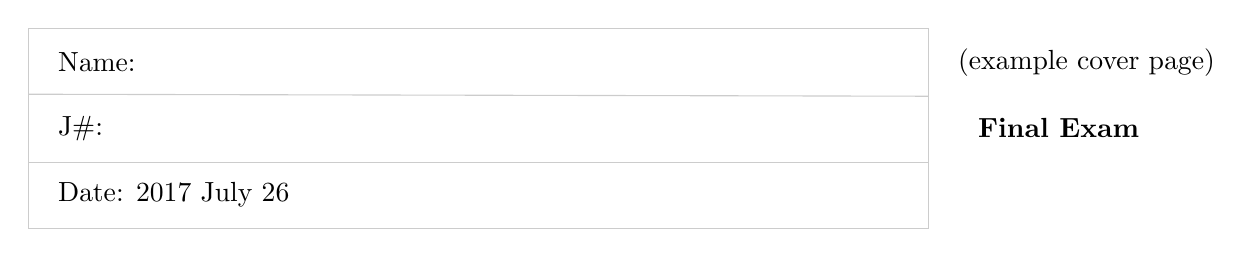
\begin{tikzpicture}[x=1in,y=1in]
  \draw[color=black!20] (0,0) rectangle (4.5,1);
  \draw[color=black!20] (0,0.67) -- (4.5,0.66);
  \draw[color=black!20] (0,0.33) -- (4.5,0.33);
quiz-20170619
  \node[anchor=west] at (0.1,0.83) {Name:};
  \node[anchor=west] at (0.1,0.5) {J\#:};
  \node[anchor=west] at (0.1,0.17) {Date: 2017 July 26};

  \node[anchor=west] at (4.6,0.83) {(example cover page)};
  \node[anchor=west] at (4.7,0.5) {\textbf{Final Exam}};
\end{tikzpicture}

\vspace{1em}

Instructions (tentative):

\begin{itemize}
  \item \textbf{Your student ID is required to take this exam.}
  \item Do \textbf{not} separate these pages.
  \item All items other than writing utensils must be put away for the duration
        of the exam. You will be provided with an updated progress report.
  \item You have \textbf{120 minutes} to complete up to \textbf{18 exercises}
        of the 36 exercises provided in a separate packet:
        two for each Core Standard C01-C12 and one for each Supporting Standard
        S01-S12. On each page, clearly mark the Standard Code and, for
        Core Standards, the exercise letter (for example: C07b or S11).
  \item Each worked exercise will be marked with \(\times\), \(\star\), or
        \checkmark{}.
  \item Three \(\star\) marks will be converted to \checkmark{} marks.
        Students with few \(\times\) marks on quizzes since July 06
        will have one or two additional \(\star\) marks converted to
        \checkmark{} marks.
  \item All the necessary information to answer each question is provided
        on the exam.
        The proctor will not answer questions or make clarifications.
  \item When you are satisfied with your solutions, submit this packet and
        the separate exercise book to
        the proctor. Then collect your belongings and exit the classroom.
  \item \textbf{Exams not submitted to the proctor in time will not be
        graded.}
\end{itemize}

\newpage


\exerciseHeaderAnswer{}{Write the Standard code (C\#\#a or C\#\#b or S\#\#)
for the exercise you are attempting:}{}{}

\vfill

\exerciseHeaderAnswer{}{Write the Standard code (C\#\#a or C\#\#b or S\#\#)
for the exercise you are attempting:}{}{}

\vfill

\newpage


\exerciseHeaderAnswer{}{Write the Standard code (C\#\#a or C\#\#b or S\#\#)
for the exercise you are attempting:}{}{}

\vfill

\exerciseHeaderAnswer{}{Write the Standard code (C\#\#a or C\#\#b or S\#\#)
for the exercise you are attempting:}{}{}

\vfill

\newpage


\exerciseHeaderAnswer{}{Write the Standard code (C\#\#a or C\#\#b or S\#\#)
for the exercise you are attempting:}{}{}

\vfill

\exerciseHeaderAnswer{}{Write the Standard code (C\#\#a or C\#\#b or S\#\#)
for the exercise you are attempting:}{}{}

\vfill

\newpage


\exerciseHeaderAnswer{}{Write the Standard code (C\#\#a or C\#\#b or S\#\#)
for the exercise you are attempting:}{}{}

\vfill

\exerciseHeaderAnswer{}{Write the Standard code (C\#\#a or C\#\#b or S\#\#)
for the exercise you are attempting:}{}{}

\vfill

\newpage


\exerciseHeaderAnswer{}{Write the Standard code (C\#\#a or C\#\#b or S\#\#)
for the exercise you are attempting:}{}{}

\vfill

\exerciseHeaderAnswer{}{Write the Standard code (C\#\#a or C\#\#b or S\#\#)
for the exercise you are attempting:}{}{}

\vfill

\newpage


\exerciseHeaderAnswer{}{Write the Standard code (C\#\#a or C\#\#b or S\#\#)
for the exercise you are attempting:}{}{}

\vfill

\exerciseHeaderAnswer{}{Write the Standard code (C\#\#a or C\#\#b or S\#\#)
for the exercise you are attempting:}{}{}

\vfill

\newpage


\exerciseHeaderAnswer{}{Write the Standard code (C\#\#a or C\#\#b or S\#\#)
for the exercise you are attempting:}{}{}

\vfill

\exerciseHeaderAnswer{}{Write the Standard code (C\#\#a or C\#\#b or S\#\#)
for the exercise you are attempting:}{}{}

\vfill

\newpage


\exerciseHeaderAnswer{}{Write the Standard code (C\#\#a or C\#\#b or S\#\#)
for the exercise you are attempting:}{}{}

\vfill

\exerciseHeaderAnswer{}{Write the Standard code (C\#\#a or C\#\#b or S\#\#)
for the exercise you are attempting:}{}{}

\vfill

\newpage


\exerciseHeaderAnswer{}{Write the Standard code (C\#\#a or C\#\#b or S\#\#)
for the exercise you are attempting:}{}{}

\vfill

\exerciseHeaderAnswer{}{Write the Standard code (C\#\#a or C\#\#b or S\#\#)
for the exercise you are attempting:}{}{}

\vfill

\newpage


\begin{multicols}{2}

\exerciseHeader{2017 June 01}{S01: 3DSpace.}{
Plot and analyze points and vectors in three-dimensional Euclidean space.
}{1/3}

Find the magnitude \(\|\vect v\|\) and
direction \(\frac{1}{\|\vect v\|}\vect v\)
of the vector \(\vect v = 6\veci-8\veck\).

% \exerciseHeader{2017 June 02}{S01: 3DSpace.}{
% Plot and analyze points and vectors in three-dimensional Euclidean space.
% }{2/3}
%
% Sketch the vector \(\vect v=\<4,-5\>\) in the \(xy\) plane.
% Then compute \(-2\vect v\), and sketch it in the \(xy\) plane
% as well.

% \exerciseHeader{2017 June 05}{S01: 3DSpace.}{
% Plot and analyze points and vectors in three-dimensional Euclidean space.
% }{3/3}
%
% In \(xyz\) space,
% sketch the vector \(\vect v=\<1,3,0\>\), the vector \(\vect w\) pointing
% from \(\<1,3,0\>\) to \(\<1,3,4\>\), and the vector \(\vect v+\vect w\).



\exerciseHeader{2017 June 02}{S02: DotProd.}{
Compute and apply the dot product of two vectors.
}{1/3}

Find \(\cos\theta\), where \(\theta\) is the angle between the vectors
\(\<1,-2,2\>\) and \(\<3,-4,0\>\).

% \exerciseHeader{2017 June 05}{S02: DotProd.}{
% Compute and apply the dot product of two vectors.
% }{2/3}
%
% Find the work done by a force of \(6\) units over a distance of \(4\) units,
% assuming that the force vector is applied at an angle of \(\pi/3\) radians from
% the displacement vector.

% \exerciseHeader{2017 June 06}{S02: DotProd.}{
% Compute and apply the dot product of two vectors.
% }{3/3}
%
% Verify that
% \[
%   \<3,0,-2\>\cdot(\<-1,2,3\>+\<3,1,4\>)
% =
%   \<3,0,-2\>\cdot\<-1,2,3\>+\<3,0,-2\>\cdot\<3,1,4\>
% \]
% by computing both sides separately.



% \exerciseHeader{2017 June 05}{S03: CrossProd.}{
% Compute and apply the cross product of two vectors.
% }{1/3}
%
% Prove that \(\veci\times\veck=-\vecj\), either by computing the cross product
% directly, or by using
% \(\vect{v}\times\vect{w}=(\|\vect v\|\|\vect w\|\sin\theta)\vect{n}\).

% \exerciseHeader{2017 June 06}{S03: CrossProd.}{
% Compute and apply the cross product of two vectors.
% }{2/3}
%
% Prove that \(\<2,-6,4\>\) and \(\<-3,9,-6\>\) are parallel vectors.

\exerciseHeader{2017 June 07}{S03: CrossProd.}{
Compute and apply the cross product of two vectors.
}{3/3}

A force of \(6\) units is applied to a wrench at an angle of \(\pi/6\)
radians to a point \(4\) units away from a bolt.
What is the mangitude of the resulting torque?



% \exerciseHeader{2017 June 07}{C01: SurfaceEQ.}{
% Identify and sketch surfaces in three-dimensional Euclidean space.
% }{1/4}
%
% Sketch the surface \((x-4)^2+y^2+(z+3)^2=4\) in \(xyz\) space.

% \exerciseHeader{2017 June 08}{C01: SurfaceEQ.}{
% Identify and sketch surfaces in three-dimensional Euclidean space.
% }{2/4}
%
% Consider the quadric surface \(z=y^2-x^2\).
%
% \vspace{1em}
%
% First sketch six traces for the surface given by \(x=-2,x=0,x=2\) and
% \(y=-2,y=0,y=2\) in two dimensions.
%
% \vfill\vfill
%
% Then use those traces to draw a rough three-dimensional sketch of the surface.
% (This quadric surface is called a hyperbolic paraboloid.)
%
% \vfill

\exerciseHeader{2017 June 09}{C01a: SurfaceEQ.}{
Identify and sketch surfaces in three-dimensional Euclidean space.
}{3/4}

Sketch the surface \(2x+y+4z=8\).

\exerciseHeader{2017 June 12}{C01b: SurfaceEQ.}{
Identify and sketch surfaces in three-dimensional Euclidean space.
}{4/4}

Sketch the equation \(x=z^2\) first as a curve in the \(xz\) plane,
then as a surface in \(xyz\) space.



\exerciseHeader{2017 June 08}{C02a: VectFunc.}{
Model curves in Euclidean space with vector functions.
}{1/4}

Give a vector function parametrizing the line passing through
\(\<0,-2,1\>\) and parallel to the line with vector function
\(\vect r(t)=\<3-2t,5+3t,-2+4t\>\).

\exerciseHeader{2017 June 09}{C02b: VectFunc.}{
Model curves in Euclidean space with vector functions.
}{2/4}

Give a vector function parameterizing the portion of the parabola \(y=x^2+2x+1\)
beginning at \(\<-1,0\>\) and ending at \(\<3,16\>\).

% \exerciseHeader{2017 June 12}{C02: VectFunc.}{
% Model curves in Euclidean space with vector functions.
% }{3/4}
%
% Give a vector function parameterizing the line segment beginning at
% \(\<1,2,3\>\) and ending at \(\<4,0,-2\>\).

% \exerciseHeader{2017 June 13}{C02: VectFunc.}{
% Model curves in Euclidean space with vector functions.
% }{4/4}
%
% Give a vector function parameterizing the circle with center
% \(\<1,2\>\) and passing through the point \(\<-2,6\>\).



% \exerciseHeader{2017 June 09}{C03: VectCalc.}{
% Compute and apply vector function limits, derivatives, and integrals.
% }{1/4}
%
% Find the limit of \(\vect r(t)=\<\frac{\sin(t-1)}{t^2},\frac{3t^2-3t}{t^2-1}\>\)
% as \(t\) approaches \(1\).
\exerciseHeader{2017 June 12}{C03a: VectCalc.}{
Compute and apply vector function limits, derivatives, and integrals.
}{2/4}

Find a vector tangent to the curve parameterized by
\(\vect r(t)=\<\sin(t),t,\cos(t)\>\) at the point \(\<0,\pi,-1\>\).

% \exerciseHeader{2017 June 13}{C03: VectCalc.}{
% Compute and apply vector function limits, derivatives, and integrals.
% }{3/4}
%
% Find \(\int\vect r(t)\,dt\) where \(\vect r(t)=\<\cos(t),6t^2,e^t\>\).

\exerciseHeader{2017 June 14}{C03b: VectCalc.}{
Compute and apply vector function limits, derivatives, and integrals.
}{4/4}

Find \(\vect r(t)\) given \(\vect r'(t)=\<\sin t,3t^2\>\) and
\(\vect r(0)=\<-2,3\>\).

\columnbreak

\exerciseHeader{2017 June 13}{S04: Kinematics.}{
Compute and apply position, velocity, and acceleration vector functions.
}{1/3}

Recall that position in ideal projectile motion is given by
\(\vect r(t) = P_0+\vect{v}_0 t-\frac{1}{2}g\vecj t^2\) where
\(P_0\) is the initial position, \(\vect{v}_0\) is initial velocity,
and \(g\) is acceleration due to gravity.

Assume \(g=10\) meters per second squared.
Find the speed of a projectile after \(0.5\) seconds if it is launched
from the ground
with initial speed \(20\sqrt{2}\)
meters per second at an angle of \(\pi/4\) radians.

% \exerciseHeader{2017 June 14}{S04: Kinematics.}{
% Compute and apply position, velocity, and acceleration vector functions.
% }{2/3}
%
% Suppose the movement of a particle along the curve \(y=x^2\) is described
% by \(\vect r(t)=\<2t-1,4t^2-4t+1\>\). Sketch this curve and plot the point
% \(\vect r(1)\) along with its velocity and acceleration vectors
% \(\vect v(1),\vect a(1)\).

% \exerciseHeader{2017 June 15}{S04: Kinematics.}{
% Compute and apply position, velocity, and acceleration vector functions.
% }{3/3}
%
% Recall that position in ideal projectile motion is given by
% \(\vect r(t) = P_0+\vect{v}_0 t-\frac{1}{2}g\vecj t^2\) where
% \(P_0\) is the initial position, \(\vect{v}_0\) is initial velocity,
% and \(g\) is acceleration due to gravity.
%
% \vspace{1em}
%
% Assume \(g=10\) meters per second squared.
% Prove that a projectile launched from a height of \(60\) meters
% with initial velocity \(\<7,20\>\) meters per second will
% land on the ground after \(6\) seconds and travel a total of
% \(42\) meters horizontally.



\exerciseHeader{2017 June 15}{C04a: VectFuncSTNB.}{
Compute and apply the arclength parameter and TNB frame for a vector function.
}{1/4}

Find the arclength parameter \(s(t)\) for the curve given by
\(\vect r(t)=\<2t,\frac{1}{3}t^3,t^2\>\). (Hint: \(z^4+4z^2+4=(z^2+1)^2\).)

% \exerciseHeader{2017 June 16}{C04: VectFuncSTNB.}{
% Compute and apply the arclength parameter and TNB frame for a vector function.
% }{2/4}
%
% Consider the curve parametrized by \(\vect{r}(t)=\<2t,\ln(\sec (2t))\>\) for
% \(-\frac{\pi}{4}\leq t\leq\frac{\pi}{4}\).
% It follows that \(\frac{d\vect r}{dt}=\<2,2\tan (2t)\>\) and
% \(\frac{d\vect T}{dt}=\<-2\sin(2t),2\cos(2t)\>\). Compute the normal vector
% and curvature at the point on this curve where \(t=\frac{\pi}{8}\).

% \exerciseHeader{2017 June 19}{C04: VectFuncSTNB.}{
% Compute and apply the arclength parameter and TNB frame for a vector function.
% }{3/4}
%
% Suppose the unit tangent and normal vectors for a parametrized curve are given
% by \(\vect T=\frac{1}{2}\<\cos t-\sin t,\sqrt 2,\cos t+\sin t\>\) and
% \(\vect N=\frac{1}{2}\<-\sin t-\cos t,0,-\sin t+\cos t\>\).
% Find the binormal vector \(\vect B\) when \(t=\pi\).

\exerciseHeader{2017 June 20}{C04b: VectFuncSTNB.}{
Compute and apply the arclength parameter and TNB frame for a vector function.
}{4/4}

Sketch the curve \(x^2+y^2=1\). Find \(\vect T\) and \(\vect N\)
at the point \(\<\frac{\sqrt 2}{2},\frac{\sqrt 2}{2}\>\) and add them to your
sketch.



\exerciseHeader{2017 June 16}{S05: MulivarFunc.}{
Sketch and analyze the domain, level curves, and graph of a two-variable
real-valued function.
}{1/3}

Sketch the level curves for the function \(f(x,y)=\sqrt{x^2+y^2}\)
where \(k=0,1,2,3\). Then sketch a graph of the function in \(xyz\) space.

% \exerciseHeader{2017 June 19}{S05: MulivarFunc.}{
% Sketch and analyze the domain, level curves, and graph of a two-variable
% real-valued function.
% }{2/3}
%
% Graph \(f(x,y)=x^2+y^2\).

% \exerciseHeader{2017 June 20}{S05: MulivarFunc.}{
% Sketch and analyze the domain, level curves, and graph of a two-variable
% real-valued function.
% }{3/3}
%
% Sketch the domain of \(g(x,y)=\sqrt{xy}\). Then plot the four level curves where
% \(k=0,1,2,3\).



\exerciseHeader{2017 June 19}{C05a: MulivarCalc.}{
Compute and apply the partial derivatives, gradient, and directional
derivatives of a multivariable real-valued function.
}{1/4}

Find \(\nabla g\) for \(g(x,y,z)=\ln(x+z)+3xy^2\).

% \exerciseHeader{2017 June 20}{C05: MulivarCalc.}{
% Compute and apply the partial derivatives, gradient, and directional
% derivatives of a multivariable real-valued function.
% }{2/4}
%
% Find the maximal value of the directional derivative for
% the function \(f(x,y)=xe^y+y\) at the
% point \(\<1,\ln 3\>\), and the direction that yields this value.

\exerciseHeader{2017 June 21}{C05b: MulivarCalc.}{
Compute and apply the partial derivatives, gradient, and directional
derivatives of a multivariable real-valued function.
}{3/4}

Find rate of change of \(f(x,y,z)=xyz+4y^2z\) at the point
\(\<-2,1,0\>\) as the variables change in the direction of
\(\vect u =\<\frac{3}{5},0,-\frac{4}{5}\>\).

% \exerciseHeader{2017 June 22}{C05: MulivarCalc.}{
% Compute and apply the partial derivatives, gradient, and directional
% derivatives of a multivariable real-valued function.
% }{4/4}
%
% Verify the mixed derivative theorem \(f_{xz}=f_{zx}\) for
% \(f(x,y,z)=2yz-3x^2z\) by computing the second partial derivative
% both ways.



\exerciseHeader{2017 June 21}{C06a: ChainRule.}{
Apply the multivariable Chain Rule to compute derivatives and find normal
vectors.
}{1/4}

Let \(f(x,y,z)=x^2y-yz+2xz^2\) and \(\vect{r}(t)=\<2t,e^t,t+3\>\).
Use the multivariable Chain Rule by to find
\(\frac{df}{dt}\) when \(t=0\).
%
% \vfill

% \exerciseHeader{2017 June 22}{C06: ChainRule.}{
% Apply the multivariable Chain Rule to compute derivatives and find normal
% vectors.
% }{2/4}
%
% Find the normal vector to the surface \(ze^x+5xy=yz-3\) at the point
% \(\<0,2,3\>\).

\columnbreak
\exerciseHeader{2017 June 23}{C06b: ChainRule.}{
Apply the multivariable Chain Rule to compute derivatives and find normal
vectors.
}{3/4}

Let the equation \(3xy^2-2x^2=4y-3\) define \(y\) as a differentiable
function of \(x\) near the point \(\<1,1\>\). Use partial derivatives
to find the slope of the line tangent to this curve at the point \(\<1,1\>\).


% \exerciseHeader{2017 June 26}{C06: ChainRule.}{
% Apply the multivariable Chain Rule to compute derivatives and find normal
% vectors.
% }{4/4}
%
% Find an equation for the plane tangent to the graph of \(f(x,y)=4xy\) at the
% point \(\<1,-2\>\).



% \exerciseHeader{2017 June 22}{S06: Lineariz.}{
% Compute the linearization of a two-variable real-valued function at a point and
% use it for approximation.
% }{1/3}
%
% Find the linearization \(L(x,y)\) for \(f(x,y)=2x+y\sqrt{x}\) at the
% point \(\<4,-2\>\). Then use it to show that
% \(f(3.9,-1.9)\approx4.05\).

% \exerciseHeader{2017 June 23}{S06: Lineariz.}{
% Compute the linearization of a two-variable real-valued function at a point and
% use it for approximation.
% }{2/3}
%
% Find the linearization \(L(x,y)\) for \(f(x,y)=ye^{xy}\) at the
% point \(\<0,2\>\). Then use it to show that
% \(f(-0.01,2.03)\approx 1.99\).
% (Hint: Don't forget to use the product rule to find \(f_y\).)

% \exerciseHeader{2017 June 26}{S06: Lineariz.}{
% Compute the linearization of a two-variable real-valued function at a point and
% use it for approximation.
% }{3/3}
%
% Find the linearization \(L(x,y)\) for \(f(x,y)=\sin(xy)\) at the
% point \(\<3,0\>\). Then use it to show that
% \(f(2.99,0.01)\approx0.03\).



% \exerciseHeader{2017 June 26}{S07: Optimiz.}{
% Use the first-derivative test and Lagrange multipliers to optimize a
% real-valued multivariable function.
% }{1/3}
%
% Find the maximum value of the function \(f(x,y)=3-x^2-y^2+2y\) on
% the closed and bounded half-disk \(0\leq y\leq\sqrt{4-x^2}\).

% \exerciseHeader{2017 June 27}{S07: Optimiz.}{
% Use the first-derivative test and Lagrange multipliers to optimize a
% real-valued multivariable function.
% }{2/3}
%
% Find the area of the largest rectangle with one corner at the origin,
% and the opposite corner at a point \(\<x,y\>\) on the circle \(x^2+y^2=8\)
% within the first quadrant (where \(x,y\) are both positive).

% \exerciseHeader{2017 June 28}{S07: Optimiz.}{
% Use the first-derivative test and Lagrange multipliers to optimize a
% real-valued multivariable function.
% }{3/3}
%
% Find three real numbers \(x,y,z\) that add to \(9\) and
% minimize the value of \(x^2+y^2+z^2\).



% \exerciseHeader{2017 July 03}{C07: DoubleInt.}{
% Compute and apply double integrals.
% }{1/4}
%
% Evaluate \(\iint_R 5xy\,dA\) where \(R\) is the rectangle where
% \(0\leq x\leq 2\) and \(1\leq y\leq 3\).

\exerciseHeader{2017 July 05}{C07a: DoubleInt.}{
Compute and apply double integrals.
}{2/4}

Change the order of integration for the integral
\(\int_0^9\int_{\sqrt{y}}^3 \cos(x^3)\,dx\,dy\).
(Do not solve this integral.)

% \exerciseHeader{2017 July 06}{C07: DoubleInt.}{
% Compute and apply double integrals.
% }{3/4}
%
% Find \(\int_1^3\int_{x}^{2x}4xy\,dy\,dx\).

\exerciseHeader{2017 July 07}{C07b: DoubleInt.}{
Compute and apply double integrals.
}{4/4}

Give an expression involving an iterated integral that equals
the average value of the function \(f(x,y)=xy^2\) over the
rectangle where \(0\leq x\leq 2\) and
\(1\leq y\leq 4\). (Do not solve this integral.)

% \exerciseHeader{2017 July 25}{C07: DoubleInt.}{
% Compute and apply double integrals.
% }{}
%
% Find a double iterated integral that equals
% the area of the region bounded by \(y=2x\) and \(y=x^2\).
% (Do not solve this integral.)



\exerciseHeader{2017 July 05}{C08a: TripleInt.}{
Compute and apply triple integrals.
}{1/4}

Express the volume of the solid \(D\)
in the first octant (where \(x,y,z\) are all
non-negative) bounded by the plane \(x+y+z=2\) as a triple iterated
integral. (Do not solve this integral.)

% \exerciseHeader{2017 July 06}{C08: TripleInt.}{
% Compute and apply triple integrals.
% }{2/4}
%
% Express \(\iiint_D(4x-3yz)\,dV\) as a triple iterated integral,
% where \(D\) is the solid above the plane \(x+y+z=4\), below
% the plane \(x+y+z=9\), and
% with \(x,y\) values inside the triangle with vertices \(\<-1,1\>\),
% \(\<-1,-1\>\), and \(\<1,-1\>\). (Do not solve this integral.)

% \exerciseHeader{2017 July 07}{C08: TripleInt.}{
% Compute and apply triple integrals.
% }{3/4}
%
% Find \(\int_1^4\int_0^2\int_0^{\sqrt y}z\,dz\,dx\,dy\).

\exerciseHeader{2017 July 10}{C08b: TripleInt.}{
Compute and apply triple integrals.
}{4/4}

Let \(D\) be the solid where \(0\leq z\leq\sqrt{4-x^2-y^2}\).
Express \(\iiint_D xy\,dV\) as a triple iterated integral
of the variables \(x,y,z\). (Do not solve this integral.)



% \exerciseHeader{2017 July 10}{S08: TransVar.}{
% Compute and apply a transformation of variables.
% }{1/3}
%
% Let \(\vect{T}(u,v)=\<u+v+1,u-2v+3\>\) be the transformation from the
% unit square \(G\) with vertices \(\<0,0\>,\<1,0\>,\<1,1\>,\<0,1\>\) in the
% \(uv\) plane to the parallelogram \(R\) with vertices
% \(\<1,3\>,\<2,4\>,\) \(\<3,2\>,\<2,1\>\) in the \(xy\) plane.
% Use this tranformation to calculuate \(\iint_R(2x+y)\,dA\).

\exerciseHeader{2017 July 11}{S08: TransVar.}{
Compute and apply a transformation of variables.
}{2/3}

Find an affine transformation from the unit square with vertices
\(\<0,0\>,\<1,0\>,\<1,1\>,\<0,1\>\) in the \(uv\) plane to the rectangle
with vertices
\(\<1,1\>,\<3,0\>,\<5,4\>\<3,5\>\) in the \(xy\) plane.

% \exerciseHeader{2017 July 12}{S08: TransVar.}{
% Compute and apply a transformation of variables.
% }{3/3}
%
% Let \(\vect{T}(u,v)=\<3u-v+2,3u+2v-1\>\) be the transformation from the
% unit triangle \(G\) with vertices \(\<0,0\>,\<1,0\>,\<1,1\>\) in the
% \(uv\) plane to the triangle \(R\) with vertices
% \(\<2,-1\>,\<5,2\>,\<4,4\>\) in the \(xy\) plane.
% Use this tranformation to calculuate \(\iint_R(y-x)\,dA\).



\exerciseHeader{2017 July 12}{C09a: PolCylSph}{
Apply polar, cylindrical, and spherical transformations of variables.
}{1/4}

Let \(D\) be the solid where \(0\leq z\leq\sqrt{4-x^2-y^2}\).
Express \(\iiint_D xy\,dV\) as a triple iterated integral
of either spherical or cylindrical coordinates. (Do not solve this integral.)
\columnbreak


\exerciseHeader{2017 July 13}{C09b: PolCylSph}{
Apply polar, cylindrical, and spherical transformations of variables.
}{2/4}

Find \(\iint_R\sqrt{x^2+y^2}\,dA\) where \(R\) is the circle bounded by
\(x^2+y^2=4\).

% \exerciseHeader{2017 July 14}{C09: PolCylSph.}{
% Apply polar, cylindrical, and spherical transformations of variables.
% }{3/4}
%
% Let \(D\) be portion of the solid \(x^2+y^2+z^2\leq 4\) where
% \(x,y,z\) are all non-negative.
% Rewrite the triple integral \(\iiint_D (x^2+y^2+z^2)\,dV\) as a triple
% iterated integral of either cylindrical or spherical coordinates.
% (Do not solve this integral.)

% \exerciseHeader{2017 July 17}{C09: PolCylSph.}{
% Apply polar, cylindrical, and spherical transformations of variables.
% }{4/4}
%
% Let \(D\) be the portion of the solid \(x^2+y^2\leq 9\) where
% \(0\leq z\leq 1\) and \(y\geq|x|\).
% Rewrite the triple integral \(\iiint_D x\,dV\) as a triple
% iterated integral of cylindrical coordinates.
% (Do not solve this integral.)

% \exerciseHeader{2017 July 25}{C09: PolCylSph.}{
% Apply polar, cylindrical, and spherical transformations of variables.
% }{}
%
% Express the volume of the sphere \(x^2+y^2+z^2=49\) as a triple iterated
% integral of either cylindrical or spherical coordinates.
% (Do not solve this integral.)



% \exerciseHeader{2017 July 14}{C10: VectField.}{
% Analyze vector fields, including computing curl and divergence.
% }{1/4}
%
% Find the curl and divergence of the vector field
% \(\vect F(x,y)=\<x-2y,3x+4y\>\).

% \exerciseHeader{2017 July 17}{C10: VectField.}{
% Analyze vector fields, including computing curl and divergence.
% }{2/4}
%
% Find the curl and divergence of the vector field
% \(\vect F(x,y)=\<xz,2xy,4xz\>\). Then compute the curl and divergence
% of the vector field at the point \(\<0,-1,2\>\).

% \exerciseHeader{2017 July 18}{C10: VectField.}{
% Analyze vector fields, including computing curl and divergence.
% }{3/4}
%
% Find the curl and divergence of the vector field
% \(\vect F(x,y,z)=\<x+z^2,y+x^2,z+y^2\>\). Then compute the curl and divergence
% of the vector field at the point \(\<3,-2,1\>\).

% \exerciseHeader{2017 July 19}{C10: VectField.}{
% Analyze vector fields, including computing curl and divergence.
% }{4/4}
%
% Find the curl and divergence of the vector field
% \(\vect F(x,y,z)=x^2y\veci+3\vecj-z\veck\). Then compute the curl and
% divergence of the vector field at the point \(2\vecj\).


\exerciseHeader{2017 July 17}{C10a: VectField.}{
Analyze vector fields, including computing curl and divergence.
}{2/4}

Find the curl and divergence of the vector field
\(\vect F(x,y)=\<xyz,4xz,2xy\>\). Then compute the curl and divergence
of the vector field at the point \(\<1,1,1\>\).

\exerciseHeader{2017 July 17}{C10b: VectField.}{
Analyze vector fields, including computing curl and divergence.
}{2/4}

Find the curl and divergence of the vector field
\(\vect F(x,y)=\veci+x^2\vecj-y\veck\). Then compute the curl and divergence
of the vector field at the point \(3\veck\).



\exerciseHeader{2017 July 18}{C11a: LineInt.}{
Compute and apply line integrals.
}{1/4}

Find the circulation of the vector field \(\vect F=\<-y,x+1\>\)
counter-clockwise around the circle \(x^2+y^2=4\).

\exerciseHeader{2017 July 19}{C11b: LineInt.}{
Compute and apply line integrals.
}{2/4}

Rewrite \(\int_C xy\,ds\) as a definite integral with respect to \(t\),
where \(C\) is the portion of the parabola \(y=x^2\) starting at \(\<3,9\>\)
and ending at \(\<-2,4\>\).
(Do not solve this integral.)

% \exerciseHeader{2017 July 20}{C11: LineInt.}{
% Compute and apply line integrals.
% }{3/4}
%
% Recall that if \(C\) is oriented counter-clockwise, then flux may be computed
% with the line integral \(\int_C\vect F\cdot\vect{n}\,ds=\int_C(M\,dy-N\,dx)=
% \int_{t=a}^{t=b}(M\frac{dy}{dt}-N\frac{dx}{dt})\,dt\).
% Find the flux of the vector field
% \(\vect F=\<x^2,xy\>\) around the circle \(x^2+y^2=16\).

% \exerciseHeader{2017 July 21}{C11: LineInt.}{
% Compute and apply line integrals.
% }{4/4}
%
% Calculate \(\int_C\<y,2x\>\cdot\vect{T}\,ds\) where \(C\) is the parabolic
% arc \(y=x^2\) from \(\<-1,1\>\) to \(\<2,4\>\).

% \exerciseHeader{2017 July 25}{C11: LineInt.}{
% Compute and apply line integrals.
% }{}
%
% Rewrite \(\int_C yz\,ds\) as a definite integral with respect to \(t\),
% where \(C\) is the line segment beginning at \(\<3,2,1\>\) and ending at
% \(\<0,2,5\>\).
% (Do not solve this integral.)



\exerciseHeader{2017 July 19}{C12a: FundThmLine.}{
Apply the Fundamental Theorem of Line Integrals.
}{1/4}

Find \(\int_C\vect F\cdot d\vect r\) where \(\vect F=\<y^2z,2xzy,xy^2\>\)
and \(C\) is an unknown curve that begins at \(\<2,2,1\>\) and ends at
\(\<-1,0,4\>\).

% \exerciseHeader{2017 July 20}{C12: FundThmLine.}{
% Apply the Fundamental Theorem of Line Integrals.
% }{2/4}
%
% Find \(\int_C\vect F\cdot d\vect r\) where
% \(\vect F=\<e^{x+2z}+4y^2,8xy,2e^{x+2z}-3\>\)
% and \(C\) is the elliptical curve formed by the intersection of the
% cylinder \(y^2+z^2=7\) and the plane \(3x+2y-\sqrt{3}z=\pi\).
% (Hint: what's the only important property of the curve?)

\exerciseHeader{2017 July 21}{C12b: FundThmLine.}{
Apply the Fundamental Theorem of Line Integrals.
}{3/4}

Compute the work done by the force vector field
\(\<\cos(x+2z)+e^y,xe^y,2\cos(x+2z)\>\)
along any path that begins and ends at the same point.

% \exerciseHeader{2017 July 24}{C12: FundThmLine.}{
% Apply the Fundamental Theorem of Line Integrals.
% }{4/4}
%
% Find \(\int_C\<2x,z,y\>\cdot\,d\vect{r}\) where \(C\) is the curve
% parametrized by \(\vect{r}(t)=\<\sqrt{8t},2^t,t^2-2t+1\>\)
% for \(0\leq t\leq 2\).



% \exerciseHeader{2017 July 20}{S09: ParamSurf.}{
% Parametrize surfaces in three-dimensional Euclidean space.
% }{1/3}
%
% Use the spherical coordinate transformation
% \(\vect{s}(\rho,\phi,\theta)=\<\rho\sin\phi\cos\theta,
% \rho\sin\phi\sin\theta,\rho\cos\phi\>\) to find a parametrization
% \(\vect{r}(\phi,\theta)\) for the hemispherical
% surface \(x=\sqrt{4-y^2-z^2}\). You may orient this surface however
% you like, but make sure to give appropriate bounds for \(\phi,\theta\).

% \exerciseHeader{2017 July 21}{S09: ParamSurf.}{
% Parametrize surfaces in three-dimensional Euclidean space.
% }{2/3}
%
% Use the cylindrical coordinate transformation
% \(\vect{c}(r,\theta,z)=\<r\cos\theta,r\sin\theta,z\>\) to find a parametrization
% \(\vect{r}(r,\theta)\) for the conical surface \(z=\sqrt{x^2+y^2}\) inside
% the cylinder \(x^2+y^2=25\). You may orient this surface however
% you like, but make sure to give appropriate bounds for \(r,\theta\).

\exerciseHeader{2017 July 24}{S09: ParamSurf.}{
Parametrize surfaces in three-dimensional Euclidean space.
}{3/3}

Parameterize the portion of the surface \(z=y^2-x^2\) above the
square \(0\leq x\leq 3\), \(1\leq y\leq 4\).

\columnbreak

% \exerciseHeader{2017 July 21}{S10: SurfInt.}{
% Compute and apply surface integrals.
% }{1/3}
%
% The function \(\vect{r}(x,y)=\<x,y,x^2+y^2\>\) parametrizes the
% elliptical paraboloid \(z=x^2+y^2\). Give a double iterated integral
% equal to the area of this surface where \(0\leq x\leq 3\) and
% \(0\leq y\leq 3\). (Do not simplify or solve this integral.)

\exerciseHeader{2017 July 24}{S10: SurfInt.}{
Compute and apply surface integrals.
}{2/3}

The function \(\vect{r}(\theta,z)=\<2\cos\theta,2\sin\theta,z\>\) parametrizes
the cylinder \(x^2+y^2=4\). Let \(S\) be the portion of the cylinder
\(x^2+y^2=4\) where \(1\leq z\leq 4\) and \(x\geq 0\).
Express the surface integral
\(\iint_S (x^2+y^2)\,d\sigma\) as a double iterated integral
of \(\theta\) and \(z\). (Do not solve this integral.)

% \exerciseHeader{2017 July 25}{S10: SurfInt.}{
% Compute and apply surface integrals.
% }{}
%
% The function \(\vect{r}(u,v)=\<1-u+3v,2-2u+v,3+u-v\>\) where
% \(0\leq u\leq 1\) and \(0\leq v\leq 1\) parametrizes the parallelogram \(S\)
% with vertices
% \(\<1,2,3\>,\<-1,0,4\>,\<2,1,3\>,\<4,3,2\>\), oriented in the direction
% of \(\<\frac{1}{\sqrt{18}},\frac{1}{\sqrt{18}},\frac{4}{\sqrt{18}}\>\).
% Compute the flux
% \(\iint_S \vect F\cdot\vect{n}\,d\sigma\) where \(\vect F=\<x+z,4,y\>\).



% \exerciseHeader{2017 July 24}{S11: GreenStokes.}{
% Apply Green's Theorem and Stokes's Theorem.
% }{}
%
% Green's Theorem states that if the boundary \(\partial R\) of a
% 2D region \(R\) is oriented counter-clockwise,
% then circulation may be computed as \(\int_{\partial R}\vect F\cdot d\vect{r}=
% \iint_R\curl\vect F\cdot\vect{k}\,dA\).
%
% Let \(C\) be the closed loop consisting of the line segments connecting
% \(\<0,0\>\) to \(\<2,0\>\) to \(\<2,2\>\) back to \(\<0,0\>\).
% Rewrite \(\int_C \<xy,3y^2\>\cdot d\vect{r}\) as a double iterated
% integral. (Do not solve this integral.)

\exerciseHeader{2017 July 25}{S11: GreenStokes.}{
Apply Green's Theorem and Stokes's Theorem.
}{}

Green's Theorem states that if the boundary \(\partial R\) of a
2D region \(R\) is oriented counter-clockwise,
then circulation may be computed as \(\int_{\partial R}\vect F\cdot d\vect{r}=
\iint_R\curl\vect F\cdot\vect{k}\,dA\).

Let \(C\) be the boundary of the triangle bounded by \(y=x,y=2x,y=4\)
oriented counter-clockwise. Express the circulation of the vector field
\(\<x^2y,x+y\>\) around \(C\) as a double iterated integral.
(Do not solve this integral.)

\columnbreak



% \exerciseHeader{2017 July 24}{S12: DivThm.}{
% Apply the Divergence Theorem.
% }{}
%
% The Divergence Theorem states that if \(\partial R\) is the boundary of a
% 2D region \(R\),
% then flux may be computed as \(\int_{\partial R}\vect F\cdot\vect{n}\,ds=
% \iint_R\dv\vect F\,dA\).
%
% Let \(C\) be the closed loop consisting of the line segments connecting
% \(\<0,0\>\) to \(\<2,0\>\) to \(\<2,2\>\) back to \(\<0,0\>\).
% Rewrite \(\int_C \<xy,3y^2\>\cdot \vect{n}\,ds\) as a double iterated
% integral. (Do not solve this integral.)

\exerciseHeader{2017 July 25}{S12: DivThm.}{
Apply the Divergence Theorem.
}{}

The Divergence Theorem states that if \(\partial D\) is the outward-oriented
boundary of a 3D solid \(D\),
then flux may be computed as \(\iint_{\partial D}\vect F\cdot\vect{n}\,d\sigma=
\iiint_D\dv\vect F\,dV\).

Let \(D\) be the cube where \(1\leq x\leq 2\),  \(0\leq y\leq 1\),
and \(3\leq z\leq 4\).
Express the flux
\(\iint_{\partial D} \<x^2,4yz,3xz\>\cdot \vect{n}\,d\sigma\) as a triple
iterated integral. (Do not solve this integral.)
\end{multicols}
\end{document}
